\pdfminorversion=4
%\documentclass[handout,xcolor=svgnames]{beamer}
\documentclass[presentation,xcolor=svgnames,aspectratio=169]{beamer}

% -*- coding: utf-8 -*-
%UTF-8: äöüß
% !TEX root = ./main.tex
%preface.tex

\usepackage[utf8]{inputenc}
\usepackage[T1]{fontenc}
\usepackage[english,ngerman]{babel}
\usepackage{color}
\usepackage{graphicx}
\usepackage{rotating}
\usepackage{xspace} 
\usepackage{epstopdf}
\usepackage{hyperref}
\usepackage{pmat}
\usepackage{tikz}
\usetikzlibrary{positioning}
\usetikzlibrary{shapes}

\usepackage{multicol}
\usepackage{algorithm}
\usepackage{algpseudocode}
\renewcommand{\algorithmicrequire}{\textbf{Input:}}
\renewcommand{\algorithmicensure}{\textbf{Output:}}
\floatname{algorithm}{Algorithmus}
% declaration of the new block
\algblock{ParDo}{EndParDo}
% customising the new block
\algnewcommand\algorithmicparfor{\textbf{for}}
\algnewcommand\algorithmicpardo{\textbf{pardo}}
\algnewcommand\algorithmicendparfor{\textbf{end\ pardo}}
\algrenewtext{ParDo}[1]{\algorithmicparfor\ #1\ \algorithmicpardo}
\algrenewtext{EndParDo}{\algorithmicendparfor}

%%%Einige Einstellungen
\mode<presentation>
{
    \usetheme{CambridgeUS}
    % \usecolortheme[named=DarkGreen]{structure}
    \usecolortheme{seahorse}
    \useinnertheme{default}
    \useoutertheme{infolines}

    % Disable navigation bar
    \setbeamertemplate{navigation symbols}{}

    %\setbeamercovered{transparent}
}


\title{NeuGenGo}
\subtitle{Kann unser neuronales Netz besser Go spielen als wir?}

\author[L. Braun, A. Schaare, T. Eimer]{Lennart Braun, Armin Schaare, Theresa Eimer}

\institute[]
    {Universität Hamburg\\ 
    Fakultät für Mathematik, Informatik und Naturwissenschaften\\
    Fachbereich Informatik, Arbeitsbereich WR\\
    Praktikum Parallele Programmierung SS 15}

\date{9. September 2015}

% PDF Dokumentinformationen: autorenspezifisch
\hypersetup {
    pdfauthor={Lennart Braun, Armin Schaare, Theresa Eimer},
    % pdftitle={\title},
    pdftitle = {\title -- \subtitle},
    pdfsubject = {Universität Hamburg / MIN / FB18 / WR / Praktikum Parallele Programmierung / SS 15},
    pdfkeywords = {parallel programming, neural networks, go},
    plainpages = false, 
    pdfstartpage = {1},
    pdfpagelabels,
    breaklinks = {true},
}

%\usepackage[style=alphabetic, backend=biber]{biblatex}
%\addbibresource{../parallele-algorithmen.bib}

\begin{document}

\maketitle

%\section{Die Idee}
%Was es tun soll, wieso wir das machen, eine kurze Einleitung eben
Neuronale Netze wurden in den letzten Jahren immer wieder für verschiedene
Problemstellungen benutzt. Es wurde festgestellt, dass sie auch komplizierte
Aufgaben lösen können, vorausgesetzt sie werden gut genug trainiert. Go zu
spielen ist ein sehr komplexe Aufgabe, die wir unter anderem genau aus diesem
Grund ausgewählt haben. Wegen der vielen Zugmöglichkeiten und dem mit 19x19
Punkten sehr großen Spielbrett, gibt es für Go noch keine Computer, die
Menschen deutlich übertreffen oder sogar eine perfekte Strategie spielen
können. Dieses Ziel wäre natürlich etwas hoch gegriffen, doch mit diesem
Projekt wollten wir sehen, ob sich neuronale Netze überhaupt gegenseitig so
trainieren können, dass sie bessere Ergebnisse erzielen. Dazu wurden zwei Tools
benutzt, das erste ist dafür zuständig die Netze zu erstellen und mit Hilfe von
Supervised Learning auf die Regeln von Go zu trainieren. Das zweite Tool lässt
die Netze dann gegeneinander antreten und rekombiniert sie mit Hilfe eines
genetischen Algorithmus. Die so entstandenen Netze können gespeichert werden
und auch gegen einen menschlichen Gegner antreten.

\section*{Gliederung}

%----------------------------------------------------------------------%SLIDE -
\begin{frame}
    \tableofcontents[
        subsectionstyle=show/hide,
    ]
\end{frame}
%----------------------------------------------------------------------%SLIDE -

\section{Problemstellung}

%----------------------------------------------------------------------%SLIDE -
\begin{frame}
    \frametitle{Problemstellung}
    \begin{itemize}
        \item
            Unser Ziel ist es, neuronale Netzwerke zu trainieren, sodass diese
            uns im Go schlagen können.

        \item Zwischenziel / Alternative:
            Können wir neuronale Netze so trainieren, sodass sie besser als
            zufällig erzeugte Netze spielen?
    \end{itemize}

    \hfill \\
    \hfill \\
\end{frame}
%----------------------------------------------------------------------%SLIDE -

%----------------------------------------------------------------------%SLIDE -
\begin{frame}
    \frametitle{Go}
    \begin{columns}
        \column{0.5\textwidth}
        \begin{itemize}
            \item Asiatisches Brettspiel
            \item Wird auf Brettern mit $19 \times 19$ Knoten gespielt.
            \item Ziel: Gebiet einkreisen und gegnerische Steine schlagen
            \item Spielende: wenn beide Spieler passen
        \end{itemize}
        \column{0.5\textwidth}
        \begin{figure}
            \centering
            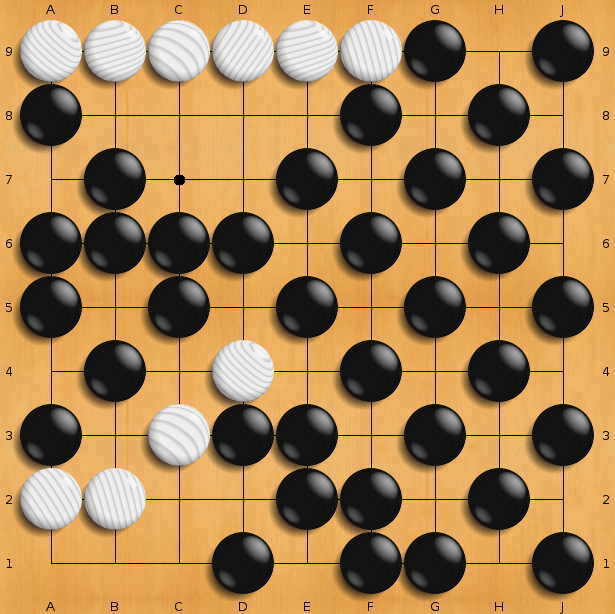
\includegraphics[scale=0.25]{content/img/go_board}
            \caption{generated with qGo}
        \end{figure}
    \end{columns}
\end{frame}
%----------------------------------------------------------------------%SLIDE -

%----------------------------------------------------------------------%SLIDE -
\begin{frame}
    \frametitle{Neuronale Netzwerke}
    \begin{itemize}
        \item Besteht aus mehreren Schichten (layer)
        \item Layer bestehen aus Neuronen
        \item Neuronen benachbarter layer sind alle durch Kanten untereinander verbunden
        \item Neuronen berechnen ihre Werte durch Aufsummieren aller eingehenden Kantengewichte multipliziert mit den Werten an den ausgehenden Neuronen
        \item Sigmoid funktion wird auf das Ergebnis angewandt, sodass alle Werte zwischen 0 und 1 sind.
    \end{itemize}
    \begin{figure}
        TODO: Graphik (möglichst unter CC / selbst erstellt)
        \caption{Schema eines neuronalen Netzwerks}
    \end{figure}
\end{frame}
%----------------------------------------------------------------------%SLIDE -

%----------------------------------------------------------------------%SLIDE -
\begin{frame}
    \frametitle{Neuronale Netzwerke}
    \begin{figure}
        \centering
        % nnet example
\begin{tikzpicture}
    [
        vertex/.style={circle, scale=1.2, draw,},
        edge/.style={-latex,},
        scale=1.5,
    ]

    \node (I1) at (0,0.5)  [vertex] {};
    \node (I2) at (0,1.5)  [vertex] {};
    \node (IT) at (0,3)    [vertex, scale=0.5] {T};
    \node (B1) at (2,0)    [vertex] {};
    \node (B2) at (2,1)    [vertex] {};
    \node (B3) at (2,2)    [vertex] {};
    \node (BT) at (2,3)    [vertex, scale=0.5] {T};
    \node (C1) at (5,0)    [vertex] {};
    \node (C2) at (5,1)    [vertex] {};
    \node (C3) at (5,2)    [vertex] {};
    \node (CT) at (5,3)    [vertex, scale=0.5] {T};
    \node (O1) at (7,0.5)  [vertex] {};
    \node (O2) at (7,1.5)  [vertex] {};

    \node at (0,4) {Input Layer};
    \node at (3.5,4) {Hidden Layer};
    \node at (7,4) {Output Layer};
    \draw [
        decorate,
        decoration={brace, amplitude=5},
    ] (-0.5,3.5) -- (0.5,3.5);
    \draw [
        decorate,
        decoration={brace, amplitude=5},
    ] (1.5,3.5) -- (5.5,3.5);
    \draw [
        decorate,
        decoration={brace, amplitude=5},
    ] (6.5,3.5) -- (7.5,3.5);

    \draw [edge] (I1) -- (B1);
    \draw [edge] (I1) -- (B2);
    \draw [edge] (I1) -- (B3);
    \draw [edge] (I2) -- (B1);
    \draw [edge] (I2) -- (B2);
    \draw [edge] (I2) -- (B3);
    \draw [edge] (IT) -- (B1);
    \draw [edge] (IT) -- (B2);
    \draw [edge] (IT) -- (B3);

    \draw [
        line width=2,
        line cap=round,
        dash pattern=on 0 off 10,
    ] (3.25,0) -- (3.75,0);
    \draw [
        line width=2,
        line cap=round,
        dash pattern=on 0 off 10,
    ] (3.25,1) -- (3.75,1);
    \draw [
        line width=2,
        line cap=round,
        dash pattern=on 0 off 10,
    ] (3.25,2) -- (3.75,2);
    \draw [
        line width=2,
        line cap=round,
        dash pattern=on 0 off 10,
    ] (3.25,3) -- (3.75,3);

    \draw [dashed] (B1) -- ($ (B1) !.33! (C1) $);
    \draw [edge, dashed] ($ (B1) !.66! (C1) $) -- (C1);
    \draw [dashed] (B1) -- ($ (B1) !.33! (C2) $);
    \draw [edge, dashed] ($ (B1) !.66! (C2) $) -- (C2);
    \draw [dashed] (B1) -- ($ (B1) !.33! (C3) $);
    \draw [edge, dashed] ($ (B1) !.66! (C3) $) -- (C3);

    \draw [dashed] (B2) -- ($ (B2) !.33! (C1) $);
    \draw [edge, dashed] ($ (B2) !.66! (C1) $) -- (C1);
    \draw [dashed] (B2) -- ($ (B2) !.33! (C2) $);
    \draw [edge, dashed] ($ (B2) !.66! (C2) $) -- (C2);
    \draw [dashed] (B2) -- ($ (B2) !.33! (C3) $);
    \draw [edge, dashed] ($ (B2) !.66! (C3) $) -- (C3);

    \draw [dashed] (B3) -- ($ (B3) !.33! (C1) $);
    \draw [edge, dashed] ($ (B3) !.66! (C1) $) -- (C1);
    \draw [dashed] (B3) -- ($ (B3) !.33! (C2) $);
    \draw [edge, dashed] ($ (B3) !.66! (C2) $) -- (C2);
    \draw [dashed] (B3) -- ($ (B3) !.33! (C3) $);
    \draw [edge, dashed] ($ (B3) !.66! (C3) $) -- (C3);

    \draw [dashed] (BT) -- ($ (BT) !.33! (C1) $);
    \draw [edge, dashed] ($ (BT) !.66! (C1) $) -- (C1);
    \draw [dashed] (BT) -- ($ (BT) !.33! (C2) $);
    \draw [edge, dashed] ($ (BT) !.66! (C2) $) -- (C2);
    \draw [dashed] (BT) -- ($ (BT) !.33! (C3) $);
    \draw [edge, dashed] ($ (BT) !.66! (C3) $) -- (C3);

    \draw [edge] (C1) -- (O1);
    \draw [edge] (C1) -- (O2);
    \draw [edge] (C2) -- (O1);
    \draw [edge] (C2) -- (O2);
    \draw [edge] (C3) -- (O1);
    \draw [edge] (C3) -- (O2);
    \draw [edge] (CT) -- (O1);
    \draw [edge] (CT) -- (O2);

\end{tikzpicture}         

        % \caption{Feedforward Netz}
        \label{fig:nnet}
    \end{figure}
\end{frame}
%----------------------------------------------------------------------%SLIDE -

\section{Lösungsansatz}

%----------------------------------------------------------------------%SLIDE -
\begin{frame}
    \frametitle{Lösungsansatz}

    \begin{itemize}
        \item Beschränkung auf $9 \times 9$ Bretter
        \item Feedforward Netze:\\
            5 Layer, mit folgender Anzahl an Neuronen: 81 82 82 82 82
        \item Genetische Algorithmen:\\
            Mutationsrate: 0.5\%\\
            Netze pro Population: 32\\
    \end{itemize}
\end{frame}
%----------------------------------------------------------------------%SLIDE -

%----------------------------------------------------------------------%SLIDE -
\begin{frame}
    \frametitle{Lösungsansatz}

    \begin{algorithm}[H]
        \caption{sequentielle Lösung}
        \begin{algorithmic}[1]
            \State $N_0 \gets \{ n$ zufällig generierte neuronale Netzwerke $\}$
            \For {$net \in N_0$}
                \State trainiere $net$ auf regelgerechtes Spielen
            \EndFor
            \For {Generation $i = 0$ bis $\ldots$}
                \For {$\forall net_a \neq net_b \in N_i$}
                    \State lass $net_a, net_b$ gegeneinander spielen
                    \State zähle die Anzahl der Siege
                \EndFor
                \State generiere $N_{i+1}$ mittels genetischen Algorithmus
                abhängig von $N_i$ und den Spielergebnissen
            \EndFor
            \State Speichere $N_n$
        \end{algorithmic}
    \end{algorithm}
\end{frame}
%----------------------------------------------------------------------%SLIDE -

%----------------------------------------------------------------------%SLIDE -
\begin{frame}
    \frametitle{UML}

    \begin{figure}
        \centering
        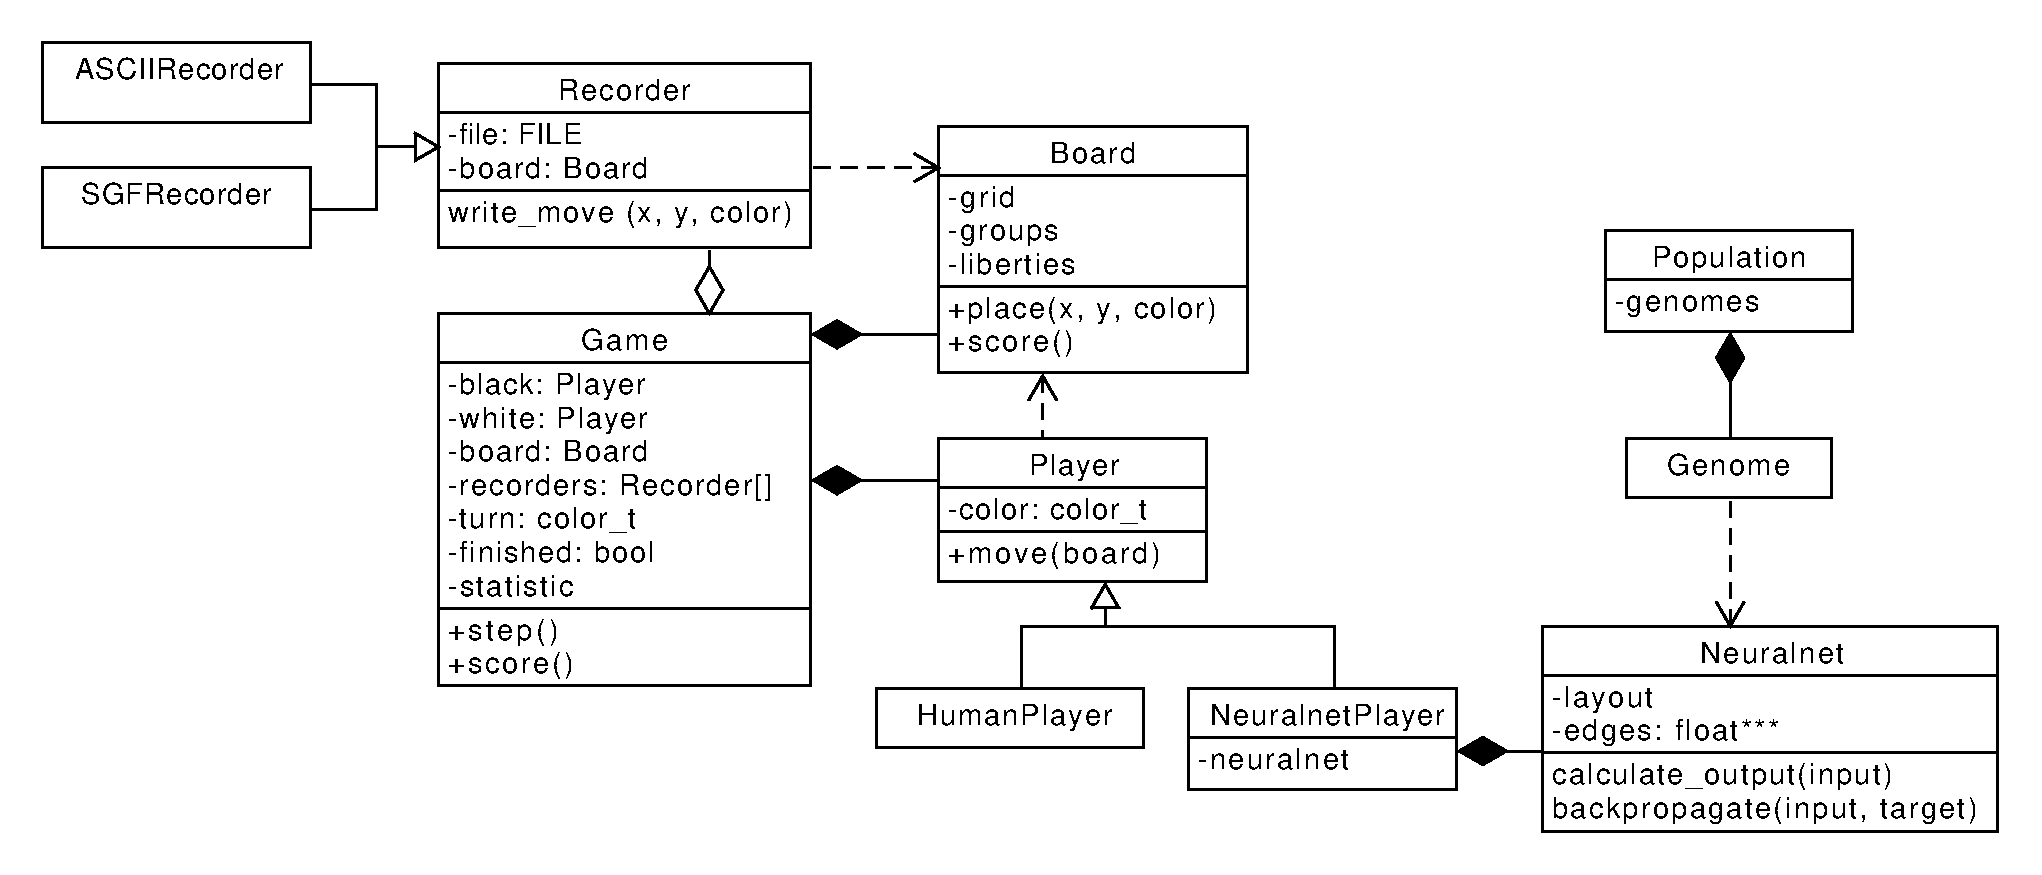
\includegraphics[scale=0.4]{content/img/class_diagram.pdf}
        \caption{Klassendiagramm}
    \end{figure}
\end{frame}
%----------------------------------------------------------------------%SLIDE -

\section{Parallelisierungsschema}

%----------------------------------------------------------------------%SLIDE -
\begin{frame}
    \frametitle{Parallelisierungsschema}

    Was ist parallelisierbar?
    \begin{itemize}
        \con
            Die Generationen sind inherent sequentiell
        \pro
            die einzelnen Spiele sind unabhängig voneinander
            (\textbf{for} $net_a, net_b \in N_i$ \textbf{do})
        \unknown
            die Ausgabeberechnung in den Neuronalen Netzwerken
            (dreifache Schleife)
    \end{itemize}
\end{frame}
%----------------------------------------------------------------------%SLIDE -

%----------------------------------------------------------------------%SLIDE -
\begin{frame}
    \frametitle{Parallelisierung der Spielphase}

    \begin{columns}[t]
        \column{0.5\textwidth}
        \vspace{-0.7cm}
        \begin{algorithm}[H]
            \caption{parallele Spielphase (1)}
            \begin{algorithmic}[1]
                \For {Generation $i = 0$ bis $\ldots$}
                    \ParDo {$\forall net_a \in N_i$}
                        \ParDo {$\forall net_b \neq net_a \in N_i$}
                            \State lass $net_a, net_b$ spielen
                            \State zähle die Siege ($wins$)
                        \EndParDo
                    \EndParDo
                    \State \Call{reduce}{$wins$}
                    \IIf {rank = 0}
                        generiere $N_{i+1}$
                    \EndIIf
                    \State \Call{broadcast}{$N_i$, 0}
                \EndFor
            \end{algorithmic}
        \end{algorithm}
        \hfill

        \column{0.5\textwidth}
        Ziel: $n^2$ Spiele auf $p$ Prozesse zu verteilen
        \begin{itemize}
            \item Master erstellt $N_{i+1}$.
            \item Master sendet $N_{i+1}$ an alle.
            \item Gleichmäßige Verteilung der inneren Schleifen (Zeilen 3,4).
        \end{itemize}
        Probleme:
        \begin{itemize}
            \item $\approx \SI{27}{\kibi\byte}$ pro Netzwerk
            \item viele kollektive Operationen
        \end{itemize}
    \end{columns}
\end{frame}
%----------------------------------------------------------------------%SLIDE -

%----------------------------------------------------------------------%SLIDE -
\begin{frame}
    \frametitle{Parallelisierung der Spielphase}

    \begin{columns}[t]
        \column{0.5\textwidth}
        \vspace{-0.7cm}
        \begin{algorithm}[H]
            \caption{parallele Spielphase (2)}
            \begin{algorithmic}[1]
                \For {Generation $i = 0$ bis $\ldots$}
                    \ParDo {$\forall net_a \in N_i$}
                        \ParDo {$\forall net_b \neq net_a \in N_i$}
                            \State lass $net_a, net_b$ spielen
                            \State zähle die Siege ($wins$)
                        \EndParDo
                    \EndParDo
                    \State \Call{reduce}{$wins$}
                    \State generiere $N_{i+1}$
                \EndFor
            \end{algorithmic}
        \end{algorithm}
        \hfill

        \column{0.5\textwidth}
        Ziel: $n^2$ Spiele auf $p$ Prozesse zu verteilen
        \begin{itemize}
            \item \emph{Jeder} erstellt $N_{i+1}$.
            \item \sout{Master sendet $N_{i+1}$ an alle.}
            \item Gleichmäßige Verteilung der inneren Schleifen (Zeilen 3,4).
        \end{itemize}
        Probleme:
        \begin{itemize}
            \item \sout{$\approx \SI{27}{\kibi\byte}$ pro Netzwerk}
            \item \sout{viele kollektive Operationen}
            \item ?
        \end{itemize}
    \end{columns}
\end{frame}
%----------------------------------------------------------------------%SLIDE -

%----------------------------------------------------------------------%SLIDE -
\begin{frame}
    \frametitle{Not So Strong Scaling}

    \begin{figure}
        \centering
        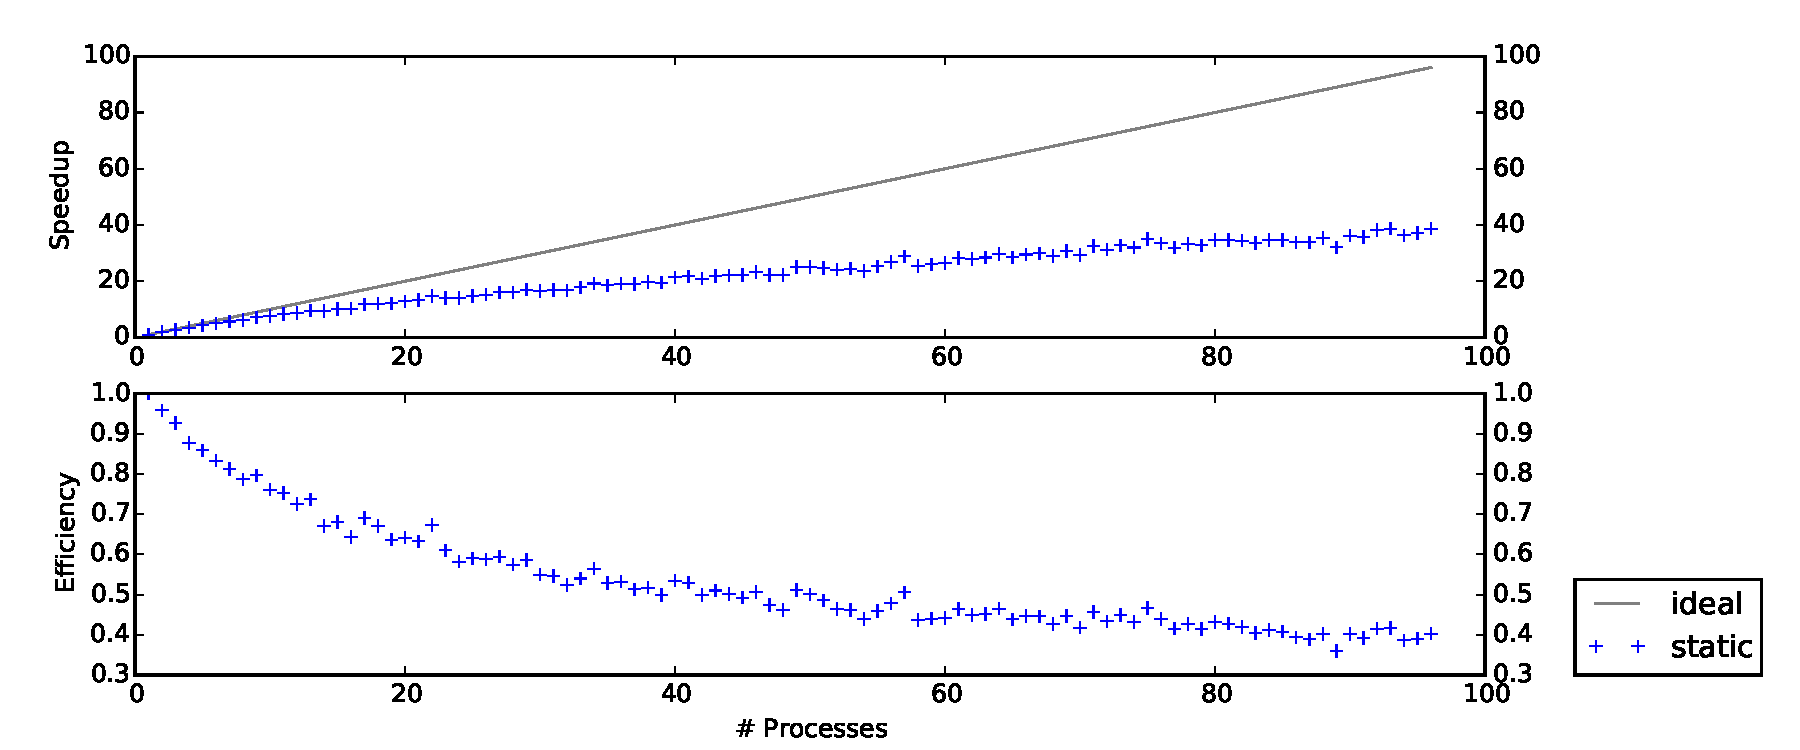
\includegraphics[width=\textwidth]{content/img/strong_scaling_time_static}
        %\caption{}
    \end{figure}

\end{frame}
%----------------------------------------------------------------------%SLIDE -

%----------------------------------------------------------------------%SLIDE -
\begin{frame}
    \frametitle{Not So Strong Scaling}
    \framesubtitle{Spurdatenanalyse}

    \begin{figure}
        \centering
        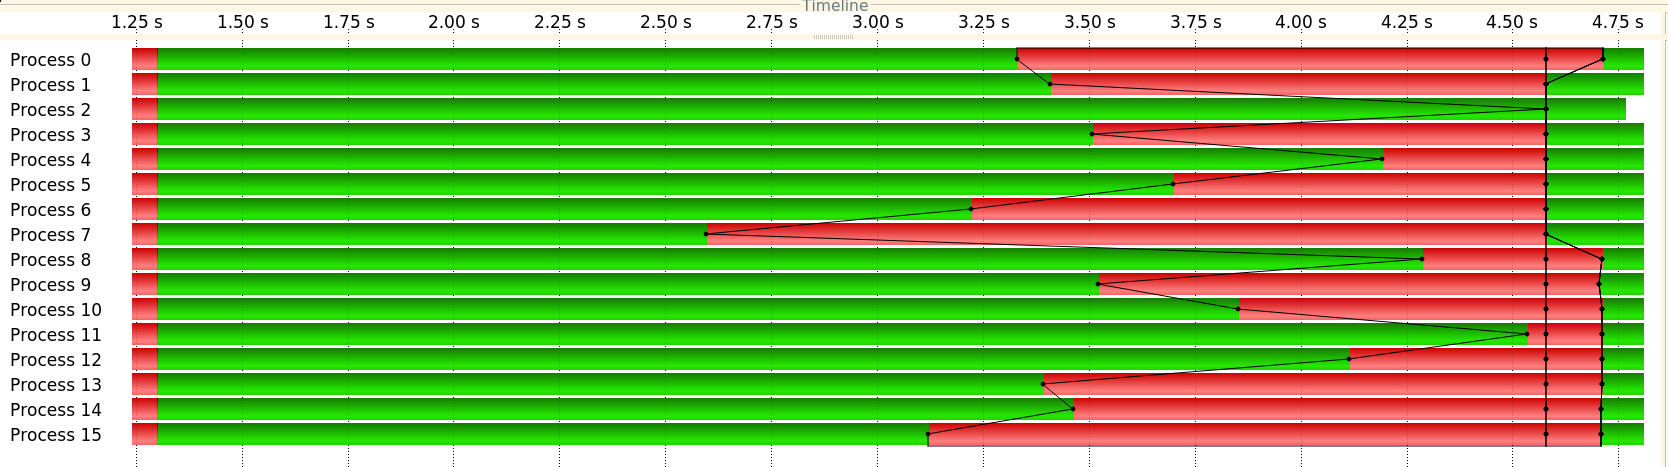
\includegraphics[width=\textwidth]{content/img/vampir_static}
        \caption{Vampir}
    \end{figure}

\end{frame}
%----------------------------------------------------------------------%SLIDE -

%----------------------------------------------------------------------%SLIDE -
\begin{frame}
    \frametitle{Not So Strong Scaling}

    Was ist da los?
    \begin{itemize}
        \item Spiele dauern unterschiedlich lange (2-1024 Züge)
        \item Länge ist nicht vorhersagbar
        \item[$\Rightarrow$] Lastungleichheit zwischen den Prozessen
    \end{itemize}

    %\pause
    \hfill

    Lösung: Dynamisches Scheduling
    \begin{itemize}
        \item Master/Worker Modell
        \item ein Anteil der Spiele wird gleichmäßig verteilt ($initial$)
        \item Master verteilt restliche Spiele paketweise an idlende Prozesse
              ($chunksize$)
    \end{itemize}

\end{frame}
%----------------------------------------------------------------------%SLIDE -

%----------------------------------------------------------------------%SLIDE -
\begin{frame}
    \frametitle{Dynamic Scheduling}

    \begin{columns}[t]
        \column{0.5\textwidth}
        \vspace{-0.7cm}
        \begin{algorithm}[H]
            \caption{Master}
            \begin{algorithmic}[1]
                \Require $initial, chunksize, n$ (number of games)
                \State $start \gets n \cdot initial$
                \While {$start < n$}
                    \State $msg, p \gets $\Call{Recv}{?}
                    \State \Call{Send}{$p, (start, chunksize)$}
                    \State $start \gets start + chunksize$
                \EndWhile
                \For {each process $p$}
                    \State $msg, p \gets $\Call{Recv}{?}
                    \State \Call{Send}{$p, (0, 0,$ "nothing to do")}
                \EndFor
            \end{algorithmic}
        \end{algorithm}

        \column{0.5\textwidth}
        \vspace{-0.7cm}
        \begin{algorithm}[H]
            \caption{Worker}
            \begin{algorithmic}[1]
                \Require initial, chunksize, number of games
                \State $start, chunksize \gets \Call{partition}{n \cdot initial}$
                \While {$chunksize \neq 0$}
                    \For {$g \in [start, start + length)$}
                        \State rechne Game $\#g$
                        \State zähle die Siege ($wins$)
                    \EndFor
                    \State \Call{Send}{$master$, "{}I'm bored"}
                    \State $start, chunksize \gets $\Call{Recv}{$master$}
                \EndWhile
            \end{algorithmic}
        \end{algorithm}
    \end{columns}
\end{frame}
%----------------------------------------------------------------------%SLIDE -

%----------------------------------------------------------------------%SLIDE -
\begin{frame}
    \frametitle{Stronger Scaling}
    \framesubtitle{Chunksize}

    \begin{figure}
        \centering
        \centering
        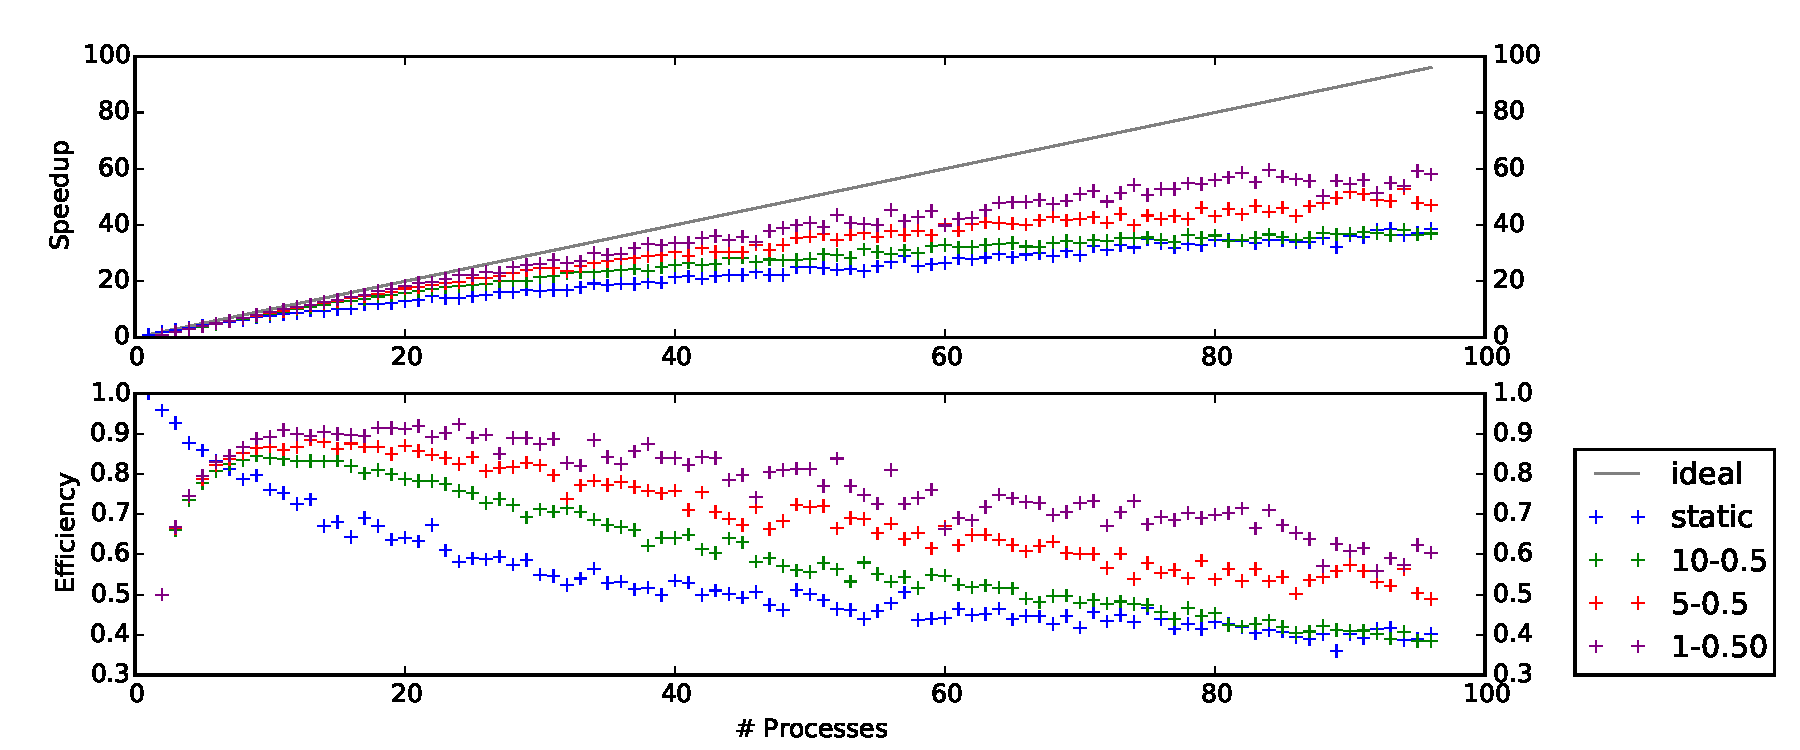
\includegraphics[width=\textwidth]{content/img/strong_scaling_time_chunksize}
        %\caption{}
    \end{figure}

\end{frame}
%----------------------------------------------------------------------%SLIDE -

%----------------------------------------------------------------------%SLIDE -
\begin{frame}
    \frametitle{Stronger Scaling}
    \framesubtitle{Initial}

    \begin{figure}
        \centering
        \centering
        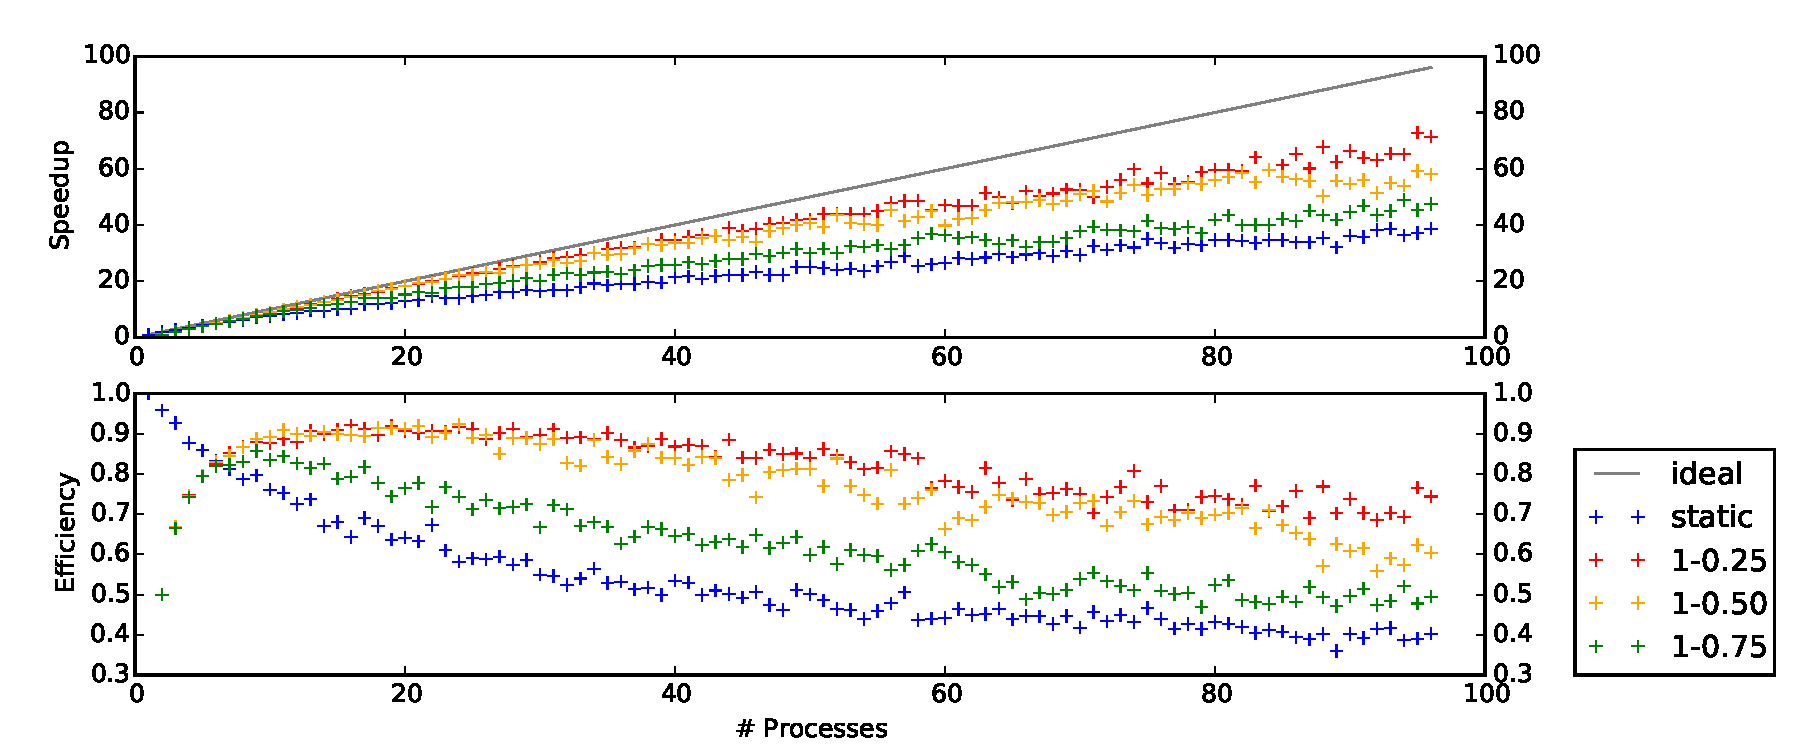
\includegraphics[width=\textwidth]{content/img/strong_scaling_time_initial}
        %\caption{}
    \end{figure}

\end{frame}
%----------------------------------------------------------------------%SLIDE -

%----------------------------------------------------------------------%SLIDE -
\begin{frame}
    \frametitle{Much Stronger Scaling}
    \framesubtitle{{}}

    \begin{figure}
        \centering
        \centering
        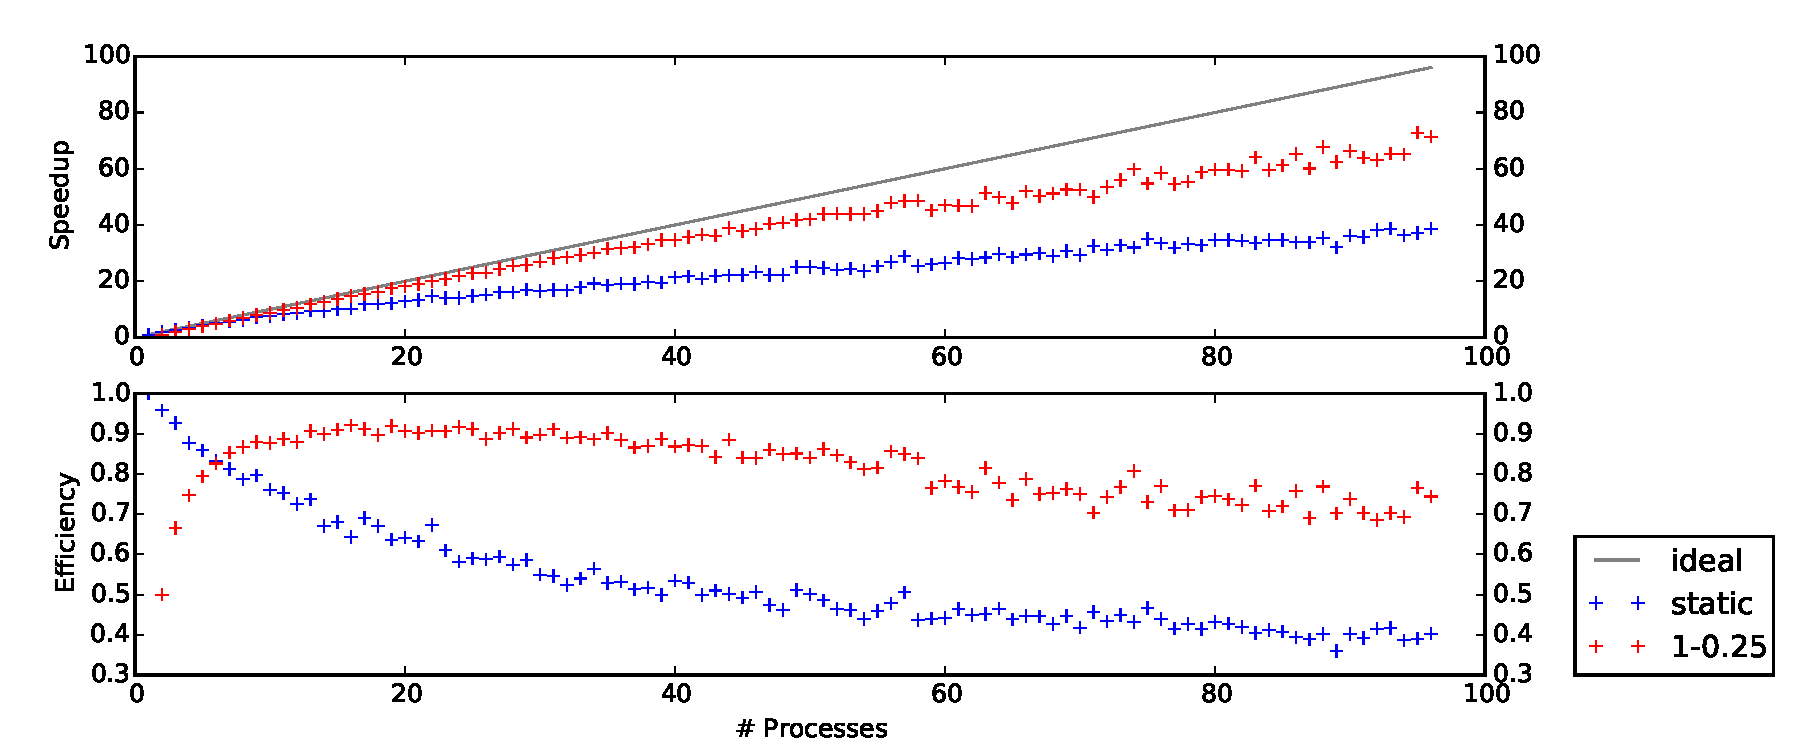
\includegraphics[width=\textwidth]{content/img/strong_scaling_time_final}
        %\caption{}
    \end{figure}

\end{frame}
%----------------------------------------------------------------------%SLIDE -

%----------------------------------------------------------------------%SLIDE -
\begin{frame}
    \frametitle{Much Stronger Scaling}
    \framesubtitle{Spurdatenanalyse}

    \begin{figure}
        \centering
        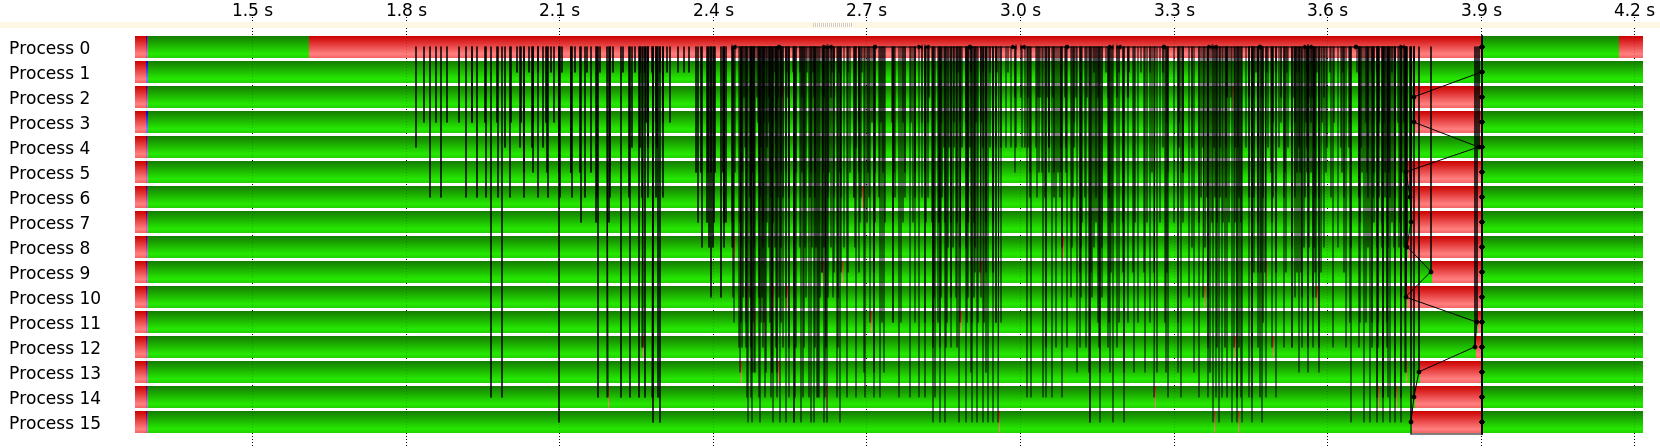
\includegraphics[width=\textwidth]{content/img/vampir_dynamic}
        \caption{Vampir}
    \end{figure}

\end{frame}
%----------------------------------------------------------------------%SLIDE -

%----------------------------------------------------------------------%SLIDE -
\begin{frame}
    \frametitle{Parallelisierung der neuronalen Netzwerke (OpenMP)}
    \begin{columns}[t]
        \column{0.6\textwidth}
        \vspace{-0.5cm}
        \begin{algorithm}[H]
            \caption{output calculation}
            \begin{algorithmic}[1]
                \Require in
                \Ensure out
                \For {each $gap$}
                    \State \Call{init}{out}
                    \ParDo {$from \gets 0$ to $neurons\_per\_layer[gap]$}
                        \For {$to \gets 0$ to $neurons\_per\_layer[gap+1]$}
                        \State $out[to] \gets out[to] +{}$
                        \State $\qquad\qquad\;\; in[from] * edges[gap][from][to]$
                        \EndFor
                    \EndParDo
                    \State \Call{swap}{in, out}
                \EndFor
            \end{algorithmic}
        \end{algorithm}
        \column{0.4\textwidth}
        \vspace{-0.5cm}
        \begin{itemize}
            \item Ist langsam.
            \item Je mehr Prozesse desto langsamer.
            \item Vermutlich zu hoher Overhead durch Fork/Join bei wenig Iterationen.
        \end{itemize}
    \end{columns}
\end{frame}
%----------------------------------------------------------------------%SLIDE -

\section{Laufzeitmessungen}

%----------------------------------------------------------------------%SLIDE -
\begin{frame}
\end{frame}
%----------------------------------------------------------------------%SLIDE -

\section{Leistungsanalyse}

%----------------------------------------------------------------------%SLIDE -
\begin{frame}
\end{frame}
%----------------------------------------------------------------------%SLIDE -

\section{Skalierbarkeit}

%----------------------------------------------------------------------%SLIDE -
\begin{frame}
\end{frame}
%----------------------------------------------------------------------%SLIDE -

%\input{content/bibliography}

\end{document}
